\documentclass[12pt]{article}%
\usepackage{amsfonts}
\usepackage{fancyhdr}
\usepackage{comment}
\usepackage[a4paper, top=2.5cm, bottom=2.5cm, left=2.2cm, right=2.2cm]%
{geometry}
\usepackage{times}
\usepackage{amsmath}
\usepackage{changepage}
\usepackage{amssymb}
\usepackage{graphicx}%
\setcounter{MaxMatrixCols}{30}
\newtheorem{theorem}{Theorem}
\newtheorem{acknowledgement}[theorem]{Acknowledgement}
\newtheorem{algorithm}[theorem]{Algorithm}
\newtheorem{axiom}{Axiom}
\newtheorem{case}[theorem]{Case}
\newtheorem{claim}[theorem]{Claim}
\newtheorem{conclusion}[theorem]{Conclusion}
\newtheorem{condition}[theorem]{Condition}
\newtheorem{conjecture}[theorem]{Conjecture}
\newtheorem{corollary}[theorem]{Corollary}
\newtheorem{criterion}[theorem]{Criterion}
\newtheorem{definition}[theorem]{Definition}
\newtheorem{example}[theorem]{Example}
\newtheorem{exercise}[theorem]{Exercise}
\newtheorem{lemma}[theorem]{Lemma}
\newtheorem{notation}[theorem]{Notation}
\newtheorem{problem}[theorem]{Problem}
\newtheorem{proposition}[theorem]{Proposition}
\newtheorem{remark}[theorem]{Remark}
\newtheorem{solution}[theorem]{Solution}
\newtheorem{summary}[theorem]{Summary}
\newenvironment{proof}[1][Proof]{\textbf{#1.} }{\ \rule{0.5em}{0.5em}}

\newcommand{\Q}{\mathbb{Q}}
\newcommand{\R}{\mathbb{R}}
\newcommand{\C}{\mathbb{C}}
\newcommand{\Z}{\mathbb{Z}}

\begin{document}

\title{Assignment 01}
\author{Student NO. 2017220159\\ Lee junha\\ https://github.com/myosoo/Assignment01.git}
\date{\today}
\maketitle

This report describes what I felt when I used github for a week. Based on this experience, I will make a github manual for me. In addition I tried to get used to LaTex.

\section{Introduction}

\subsection{What is github?}
\paragraph{}
I have never used github before. I have been downloaded open source libraries and code distribute via github, but I did not know about what github is and how to use it. Github is a web hosting service that supports projects using git. In short, it is made to change git which is configured in Text to GUI and use it conveniently. Using this github, developers shared their source and improve performance. Therefore, computer science researcher seems to be able to make it familiar with how to use github. Of course, including me. 

\subsection{Advantages}
\paragraph{}
The greatest advantage of github I felt is that very free to access the source. I don’t need to strive to gain authority to access the source. There is no registration procedure too. For example, I would like to look at denoising autoencoder code. Just I can read and change the code directly from github. This is the difference from other cloud services. Also, I can share my source with other developer and exchange opinion. Although I have not tried it yet, but I don’t doubt that I believe it is very useful for my future research activities.

Another advantage is that I can manage my projects anywhere without constraints of space. Just upload my project to github and run it on local computer. The concept of Github is different from the general cloud system. At this time, github copies the entire server repository to a local repository. Therefore, even if many people collaborate, there is no conflict.

\section{How to use github}
\subsection{Preparations}
\paragraph{}
\begin{enumerate}
\item Connect to https://github.com page
\item Sign up for github
\item Create a new repository
\item Install GitBash
\item Connect local repository with github repository\\
\# git init\\
\# git remote add origin https://github.com/myosoo/Assignment01.git\\

\end{enumerate}

\subsection{Using github}
\paragraph{}
First, I imported the file in github to the local repository using the pull command. I got the README.md file and Assignment01.tex file that I created on the web. Then I tried to upload new text file on github repository. The new text file name is test.txt. Then I was able to confirm that the new file was uploaded. And I could check the commit I added. I think it will be effective in collaborative work because I can see a log of who changed what. Also I grasped the changes on the history tab. Likewise, I used the same command to bring another git on my local computer. 

In the next step, I examined branch which is one of the most important functions of github. Confirming other git, master branch was usually used for updating the version of the project. Instead, researchers have independent branches. Ultimately, They merged each branch. I think this structure makes collaborative work among researchers more efficient.

\subsection{Command of github}
\begin{figure}[h!]
\centering
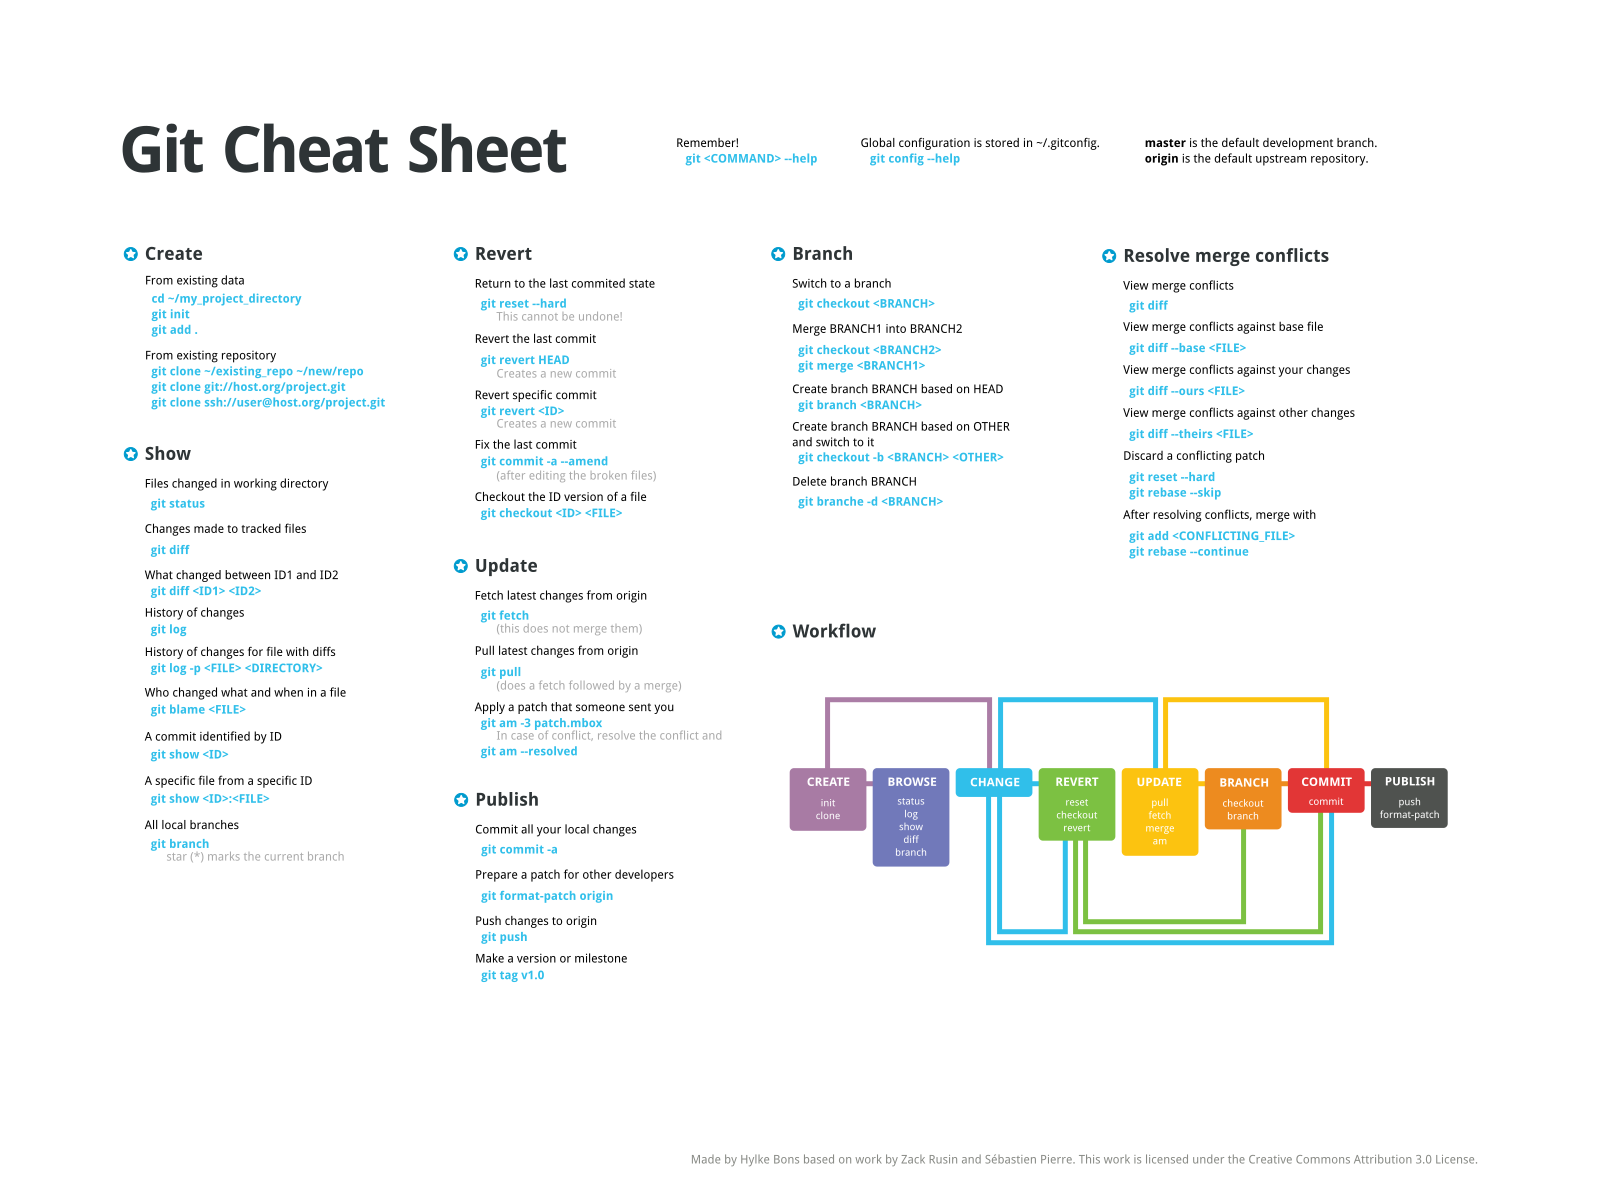
\includegraphics[scale=0.24]{github}
\caption{Github command 1}
\label{fig:Github}
\end{figure}


\section{Conclusion}
\paragraph{}
At this assignment I understood about the structure of github and how to use it. This is a very efficient and powerful tool in research and development of computer science. As a result, I confirmed that github is a very good tool to collaborate with other researchers. 

\begin{figure}[h!]
\centering
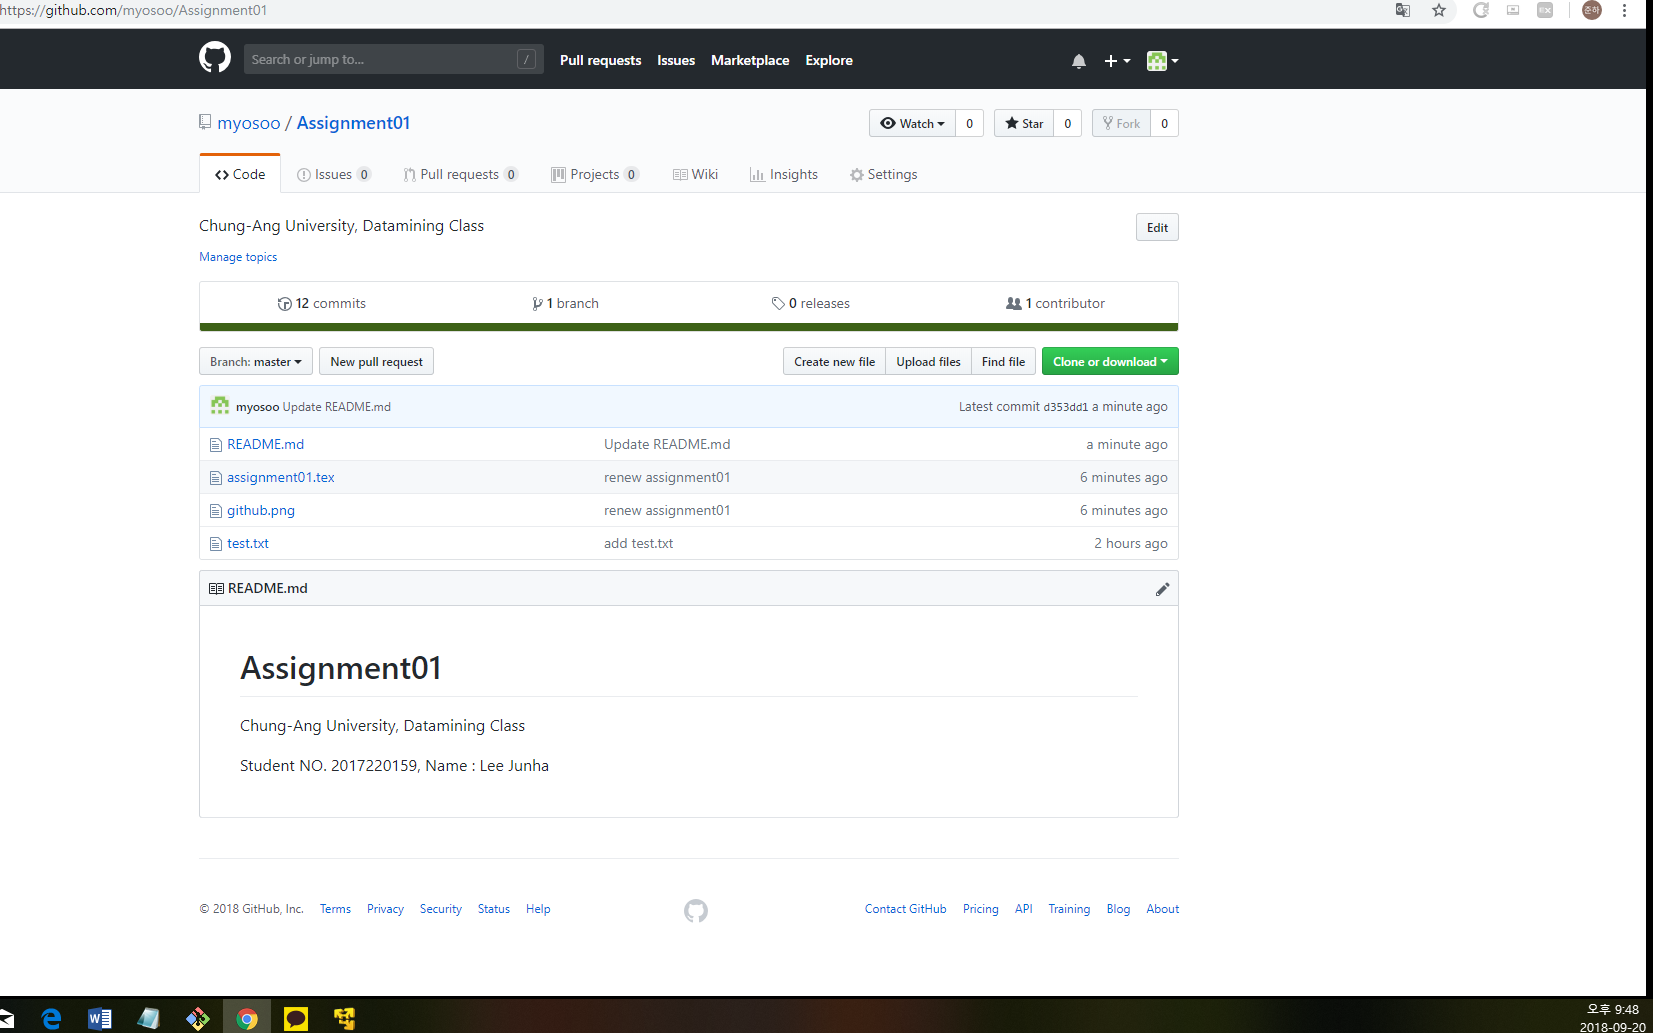
\includegraphics[scale=0.35]{screenshot}
\caption{screenshot}
\label{fig:screenshot}
\end{figure}
\end{document}